\chapter{Understanding Transformers}
\label{C:transformers}

Many of the recent amazing results in deep learning have been achieved with a class of neural networks called \textit{transformers}, which were introduced and named in "Attention Is All You Need", Vaswani et al. 2017 \cite{attention-is-all-you-need}. The distinguishing feature of these models is using one or more \textit{attention} layers to enable information propagation between elements in sequence data. Since 2017, a large number of transformer variants have been developed.

This chapter seeks to understand this class of models at a broader level, including:
\begin{itemize}
    \item The unique properties of the attention operation, which include working with sequences of any length without changing the weights, being able to be computed in parallel across the sequence during training, and being invariant to the order of the inputs.
    \item The different variants of transformers, namely encoder-only, decoder-only, and encoder-decoder models.
    \item The variety of different tasks that these model are trained on and used for, building up to the next chapter which uses transformers in their most flexible capacity.
\end{itemize}

The first and most imporant concept to understand is the operation that under-pins transformers -- attention.
\section{The Attention Operation}
\label{S:attn}

Attention is a biologically-inspired mechanism that allows a model to receive inputs from distant parts of the input data, weighted by the \textit{attention weight} given to those inputs, which is typically computed from the data itself. This has proven extremely useful for diverse tasks including machine translation, image generation, and more.

Attention has a number of useful properties which come from its mathematical construction, such as permutation-invariance in the inputs.

\subsection{Mathematical Definition}

An attention operation is of the following form, using short summation notation, where $\sigma$ is the \textit{softmax} operator (see \ref{eqn:softmax})
\begin{gather*}
    \nfdef{f_{\text{attn}}}{\R^{M×D}×\R^{N×D}×\R^{N×V}}{\R^{M×V}}
\end{gather*}
\vspace{-10pt}
\begin{equation}
\label{eqn:attn}
\begin{split}
    f_{\text{attn}}(Q, K, V)_{mv} ≝ \sum_n \left[\sigma\Big(\sum_d Q_{md} K_{nd}\Big) _{mn} V_{nv} \right]
\end{split}
\end{equation}%
\begin{gather*}
    Q ∈ \R^{M×D}, K ∈ \R^{N×D}, V ∈ \R^{N×V} \\
    M, N, D, V ∈ \N
\end{gather*}\vspace{-10pt}\\
The innermost multiplication of $Q$ and $K$ in the above equation is simply the expanded form of inner product (dot product) between vectors $Q_m$ and $K_n$. This operation however is not inherent. Instead of the inner product, we can substitute any kernel function $k(q, k)$
\begin{equation}
\label{eqn:attn-kernel}
\begin{split}
    f_{\text{attn}}(Q, K, V)_{mv} ≝ \sum_n \left[\sigma(k(Q_m, K_n)) _{mn} V_{nv} \right]
\end{split}
\end{equation}%
However, substituting a different kernel function is not usually done because the inner product is the most natural choice, and is efficient to compute.

For clarity, the expanded form of the attention computation, resulting in the unnormalized attention weights $A$, for an arbitrary kernel function $k$, is as follows:
\begin{align*}
A_{mn} = k(Q_m, K_n)
&= \begin{bmatrix}
    k(Q_{1}, K_{1}) & k(Q_{1}, K_{2}) & \cdots & k(Q_{1}, K_{N}) \\
    k(Q_{2}, K_{1}) & k(Q_{2}, K_{2}) & \cdots & k(Q_{2}, K_{N}) \\
    \vdots & \vdots & \ddots & \vdots \\
    k(Q_{M}, K_{1}) & k(Q_{M}, K_{2}) & \cdots & k(Q_{M}, K_{N})
\end{bmatrix}
\end{align*}
or, when $k(a, b)$ is chosen to be $a \cdot b$ (the inner product):
\begin{align*}
A_{mn} = k(Q_m, K_n) = Q_m \cdot K_n
&= \begin{bmatrix}
    Q_{1,1} & Q_{1,2} & \cdots & Q_D \\
    Q_{2,1} & Q_{2,2} & \cdots & Q_D \\
    \vdots & \vdots & \ddots & \vdots \\
    Q_{M,1} & Q_{M,2} & \cdots & Q_D
\end{bmatrix} \begin{bmatrix}
    K_{1,1} & K_{1,2} & \cdots & K_D \\
    K_{2,1} & K_{2,2} & \cdots & K_D \\
    \vdots & \vdots & \ddots & \vdots \\
    K_{N,1} & K_{N,2} & \cdots & K_D
\end{bmatrix}^T \\
&= Q K^T .
\end{align*}

We can see that the attention weights $A$ have shape $M×N$. This is the primary drawback of the attention operation. $M$ and $N$ are typically both large, and the attention weights take $O(MND)$ time to compute (assuming dot product attention), and $O(MN)$ space to store. Despite this drawback, the attention operation has proven extremely useful in a variety of tasks. There are many different ways to address this but they are out of scope here.

The query, key and value vectors $Q$, $K$ and $V$ are typically computed via three learned projections:
\begin{align}
\begin{aligned}
\label{eqn:attn-linear}
Q &= W_{Q} \X + \vb_{Q} \\
K &= W_{K} \X + \vb_{K} \\
V &= W_{V} \X + \vb_{V}
\end{aligned}
\end{align}
where $\X$ is a sequence of latent vectors -- either the embedded inputs to the network, or the outputs of a previous layer.

\subsection{Permutation-invariance with respect to $K$ and $V$}

The first interesting property of attention is that it is permutation-invariant with respect to the key and value inputs. This property is more or less useful depending on the task. For example, in the case of graphs, or sets of heterogeneous values, there may not be a natural ordering in which to process the inputs. In this case, we do not have to introduce any artificial ordering. (However, when \textit{sampling} outputs, we typically still need to decide on some order. This is discussed in more detail in \Cref{C:a-o-sampling}).

This property is due to the construction of the attention operator. We can see that the output $O_m$ corresponding to a query vector $Q_m$ is independent of the order of the key and value vectors $K_n$ and $V_n$, because the summation across $n$ is commutative:
\begin{align}
\label{eqn:attn-perm-invariance}
\begin{aligned}
    O_m &= \sum_n V_n \sigma(A_{m})_n
\end{aligned}
\end{align}

\subsection{Permutation-equivariance with respect to $Q$}

Relatedly, attention is also permutation-\textit{equivariant} with respect to the query inputs. Equivariance means that the value of the output $O_m$ is dependent on the value of the query vector $Q_m$, but independent of the order of all \textit{other} query vectors $Q_{m'}$, $m' ≠ m$.

For example, let us imagine we have a sequence of four key \& value inputs $[K_1, K_2, K_3, K_4]$, and $[V_1, V_2, V_3, V_4]$, and a sequence of three query inputs $[Q_A, Q_B, Q_C]$ which when passed into an attention operation, produce three outputs $[O_A, O_B, O_C]$. First, due to the first property (invariance in $K$ and $V$), if we swap for example the inputs $K_1$ \& $V_1$ with $K_3$ and $V_3$, the output sequence will remain $[O_A, O_B, O_C]$. Second, if we swap the inputs $Q_A$ and $Q_C$, the second property (equivariance in $Q$) means that the output sequence is correspondingly transformed to $[O_C, O_B, O_A]$.

This property is due to the fact that softmax operation is equivariant to the order of its inputs, which we can see from the construction in \Cref{eqn:softmax}.

This property of attention stands in contrast to the two main other methods used to process sequence data, convolution (CNNs) and recurrence (RNNs). Neither of these operations are permutation invariant or equivariant with respect to their inputs.

\subsection{Dynamic length inputs}

The second (and most useful) property of attention is that it can be used to process inputs of dynamic length. We can again see why this is the case from \Cref{eqn:attn-perm-invariance}. The softmax operation normalizes the attention weights, which causes the resulting summation of vectors $V_n$ to be a convex combination. The resulting output $O_m$ will therefore sit within the convex hull of the vectors $V_n$. This means that the output $O_m$ will be a ``valid'' output regardless of the length of the input sequence $K_v$.

\subsection{Parallel computation}

The third property of attention is that it can be computed in parallel across the inputs sequence during training. At all steps of the attention computation except the softmax operation, there are no dependencies between neighbouring elements of the tensors. This stands in contrast to RNNs, where the outputs for one position in the sequence depend on the previous outputs.

The fact that attention can be computed in parallel is a very useful property, since while the operation requires $O(MN)$ in time and space, if we can utilize bigger GPU hardware the real-time cost reduces to $O(1)$ (assuming sufficient memory capacity, compute capability, and also GPU memory bandwidth, which is often the limiting factor \cite{multi-query-attn}.) The attention logits $A_{mn}$ can be computed entirely in parallel. The softmax operation depends on all previous attention logits across the key-value dimension $N$, which requires cross-talk between GPU units but does not prevent parallel computation. The final computation for the outputs $O_m$ can also be computed in parallel.

So attention is a operation with a number of useful properties. Now we will see how it is used to build a variety of models capable of solving a variety of tasks with sequence data.

\section{Basic components of transformers.}

An attention operation model does not itself make a neural network. It is simply a building block that can be used to construct a neural network.

\subsection{Residual Blocks}

A transformer model puts attention operations together with MLP blocks similarly to in residual networks (ResNets \cite{resnet}). Without MLP blocks as non-linearities, the outputs of an attention operation are linear functions of the inputs, since the softmax is only used to compute coefficients when summing the values. Because the weights are convex (sum to 1), the output vectors of an attention operation are convex combinations of the value vectors, and will always sit within the convex hull of the value vectors. (However, note that the outputs are non-linear functions of the inputs, due to the fact that the weights are also computed from the inputs). Attention-only we would like to be able to apply non-linear transformations to the value vectors. MLP blocks are used to introduce additional non-linearities into the model.

\Cref{fig:residual-block} shows a diagram of a typical residual block in a transformer, with an attention operation, an MLP, and a residual connection.

\begin{figure}
    \centering
    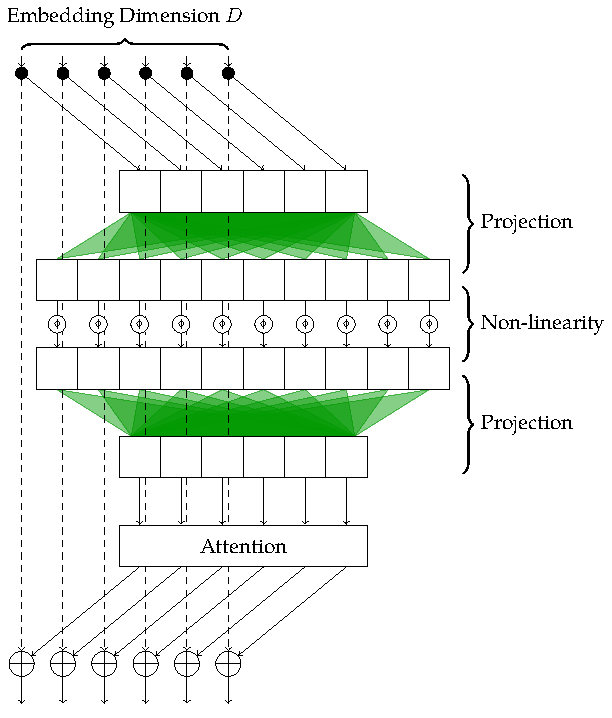
\includegraphics[]{figures/residual-block.pdf}
    \captionsetup{parskip=7pt}
    \caption[Typical residual block in transformer]{Typical residual block in transformer (with the $D$ dimension expanded, rather than the $N$ or $M$ dimension as usual.).

    In the MLP block, the sequence of residual latents are (independently) projected into a higher-dimensional space, where a non-linearity is applied, and then projected back down to the original dimensionality. Projecting to a higher dimension allows the block to represent more complex functions, and projecting back down is mostly for computational efficiency. The output of the MLP block is then projected into $Q$, $K$, and $V$ spaces, and the attention operation is applied. Finally, the results are added to the residual stream.}
    \label{fig:residual-block}
\end{figure}

\subsection{Multi-head attention}

Since the introduction of transformers it is common to use \textit{multi-head} attention, which allows for multiple \textit{heads} which each perform an attention operation in parallel with smaller key \& query dimensionality $D_{\text{head}} = \frac{D}{ n_{\text{heads}}}$.

Multi-head attention splits the key, query, and value matrices into $n_{\text{heads}}$ smaller matrices, each with dimensionality $D_{\text{head}}$, and computes $n_{\text{heads}}$ separate attention matrices. The results are then concatenated together and projected back down to the original dimensionality $D$:
\begin{align}
\begin{aligned}
\label{eqn:multi-head-attn}
Q &= W_{Q} \X + \vb_{Q} \\
K &= W_{K} \X + \vb_{K} \\
V &= W_{V} \X + \vb_{V} \\
Q_{h} &= \text{split}(Q, n_{\text{heads}}) \\
K_{h} &= \text{split}(K, n_{\text{heads}}) \\
V_{h} &= \text{split}(V, n_{\text{heads}}) \\
A_{h} &= \text{softmax}(\frac{Q_{h}K_{h}^T}{\sqrt{D_{\text{head}}}}) \\
O_{h} &= A_{h}V_{h} \\
O &= \text{concat}(O_{h}) \\
O &= W_{O}O + \vb_{O}
\end{aligned}
\end{align}
where $\text{split}$ and $\text{concat}$ are operations which split and concatenate the tensor along the $D$ dimension.

\subsection{Training task and input formats}
\label{ss:transformer-inputs}

Attention operates a sequence of latent vectors $\X$, but the input to a transformer model will not necessarily be in this format. Mapping the input into this format is the job of the embedding layer. The form of the embedding layer depends on the task being solved. For example, in language modelling, the input is provided as discrete tokens. The embedding layer is then a lookup table (also called a codebook), which maps each token to a learned vector. In timeseries data, the input is provided as a sequence of real-valued vectors. The embedding layer is then a linear transformation, which maps each vector to a learned vector.

Recall that attention is order independent. However, information about the order of inputs is often neccessary to perform a task. When order is important, the embedding layer will include an additional learned vector, which is added to the input vectors. This vector is called a \textit{positional encoding}. The two most common choices for positional encoding are sinusoidal and codebook encodings. A codebook encoding is simply a lookup table, which maps each position in the sequence to a learned vector. Sinusoidal positional encodings were introduced in the original transformer paper \cite{attention-is-all-you-need} and are vectors of ($\sin$, $\cos$) pairs of different frequencies.

To form the input embedding vectors $\X$, the embedded `content' vectors are then typically added to the embedded `position' vectors.

The next sections will introduce \textit{masking} and \textit{pretraining tasks}, which are the primary ways that transformer architecture variants differ.

\section{Masking and Pretraining}
\label{s:masking}

When transformer models are trained, they are often trained on large datasets of un-labeled data. The resulting models are then often further trained on smaller labeled datasets, which is called transfer-learning or fine-tuning.

In order to train a model on large unlabeled data, it needs to be formatted into a self-supervised learning task, (also called a pre-training task). This is done via masking out certain inputs and/or connections within the model itself. There are two types of masking, input masking and attention masking, which distinguish the two main pretraining tasks are \textit{masked sequence modeling} and \textit{auto-regressive pretraining}.

\subsection{Masked sequence modeling}
\label{ss:msm}

\begin{figure}
    \centering
    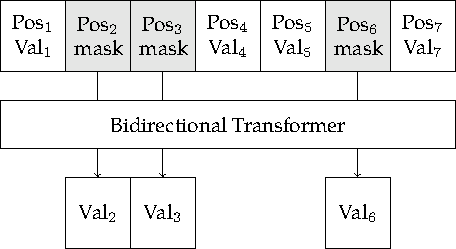
\includegraphics{figures/pretraining-msm.pdf}
    \caption[Masked Sequence Modeling Pretraining]{Masked sequence modeling pretraining task. The model is trained to reconstruct masked-out elements of the original sequence.}
    \hrulefill
    \label{fig:pretraining-msm}
\end{figure}

Masked sequence modeling is a pretraining task which uses the first kind of masking -- input masking -- to define random tasks. In this task, a random subset of sequence elements is masked out, and the model is trained to reconstruct the masked inputs. Input masking means that the `content' embedding is replaced with a `mask' embedding (which is a learned vector). The positional encoding is still provided. A diagram of this is shown in \Cref{fig:msm}.

\subsection{Causal Masking \& Auto-regressive pretraining}
\label{ss:autoreg-pretraining}

\begin{figure}
    \centering
    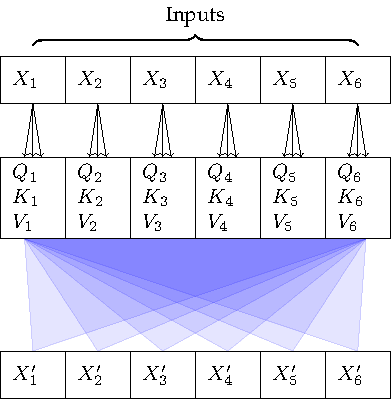
\includegraphics[]{figures/attn-1-self.pdf}
    \caption[Self-attention]{Full self-attention (bi-directional attention), as used in transformer encoders. The blue shaded regions show which inputs are used to compute each output. In full self-attention, all inputs are used to compute all outputs.}
    \label{fig:self-attn}
\end{figure}

\begin{figure}
    \centering
    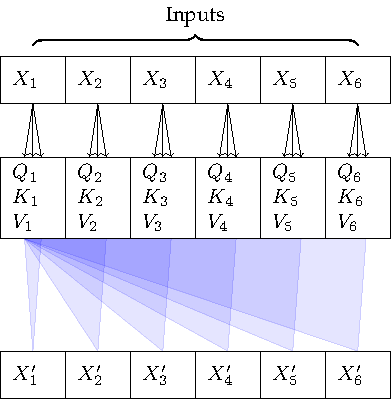
\includegraphics[]{figures/attn-3-causal.pdf}
    \caption[Self-attention with causal masking]{Self-attention with causal masking, (uni-directional attention) as used in transformer decoders during training. The blue shaded regions show which inputs are used to compute each output. In causal masking, only inputs to the left of the current output are used to compute the current output.}
    \label{fig:self-attn-causal}
\end{figure}

\begin{figure}
    \centering
    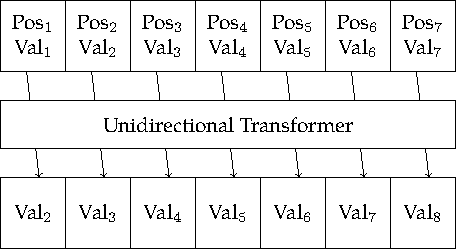
\includegraphics{figures/pretraining-causal.pdf}
    \caption[Autoregressive Sequence Modeling Pretraining]{Autoregressive pretraining task. The model is trained to predict the next element in the sequence.}
    \label{fig:pretraining-causal}
\end{figure}

\begin{figure}
    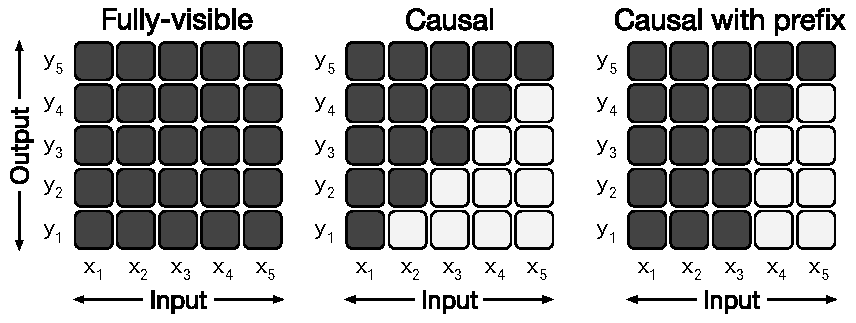
\includegraphics[width=\linewidth]{figures/attention_masks.pdf}
    \caption[Attention Masks]{Masking in unified attention layers \cite{unilm,t5}. The bi- and uni-directional attention can be performed within a single attention layer.}
    \label{fig:unified-masking}
\end{figure}

The second type of masking is \textit{attention masking}. This masking is applied to the attention operation itself. Specifically, a large constant is subtracted from the attention logits for all inputs which are to be masked out. A diagram of the different types of masking is shown in \Cref{fig:unified-masking}.

The most common use for attention masking is \textit{causal} attention masking. This masking scheme is used to define a ``forward-only'' prediction task (also called an auto-regressive task). The masking limits information to only flow in one direction through the model with respect to the sequence dimension. A diagram of causal masking is shown in \Cref{fig:self-attn-causal}.

The inputs and outputs are offset, so that the model is trained to predict the next token in the sequence. This is shown in \Cref{fig:pretraining-causal}.

Because causal masking means information only flows from left to right along the sequence, models which have only been trained on this task are called \textit{unidirectional}. In contrast, models trained on masked sequence modeling use no attention mask (which is sometimes called \textit{full} self-attention, shown in \Cref{fig:self-attn}). This allows information to flow in both directions along the sequence and so models trained with this pretraining task are called \textit{bidirectional} models.

The following chapter experiments with a new pre-training task, which is a variation on auto-regressive sequence modeling.

\subsection{Unified pretraining}
\label{ss:unified}

Input masking and attention masking can be combined arbitrarily into a single pretraining task, as we see in \Cref{fig:unified-masking}. This is called \textit{unified} pretraining / masking eg. \cite{unilm,t5}.

Unified pretraining allows the use of a model as either a bidirectional or unidirectional model, but it is costly because the attention matrix is $O((A+B)^2)$, where $A$ is the sequence of inputs that will be encoded with bidirectional attention, and $B$ is the sequence of inputs that will be encoded with unidirectional attention.

\subsection{Cross attention}
\label{ss:cross-attn}

\begin{figure}
    \centering
    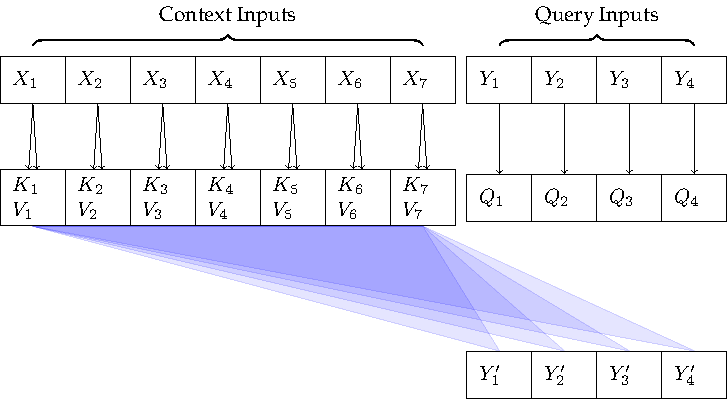
\includegraphics[]{figures/attn-2-cross.pdf}
    \caption[Cross-attention]{Cross-attention, as used in encoder-decoder models.}
    \hrulefill
    \label{fig:cross-attn}
\end{figure}

Instead of using a unified self-attention layer, it is possible to separate the dense and causal parts of the sequence into two separate layers, and connect the two with \textit{cross attention} layers, as shown in \Cref{fig:cross-attn}. This reduces the time and memory complexity of the attention matrix to $O(A^2 + B^2 + AB)$.

\section{Transformer Architectures}

When assembled into a complete model, different combinations of pretraining tasks / masking schemes / attention layers define the different transformer architectures. The next sections will introduce the four most common transformer architectures.

\subsection{Encoder-only models}
\label{ss:encoder-only}

Arguably the simplest attention-based model architecture is encoder-only transformers, which are trained on a masked sequence modeling task. Masked sequence modeling is also called Masked Language Modeling (MLM), Masked Image Modeling (MIM), etc. depending on the domain. When used in natural language processing (NLP) they are known as bi-directional language models, because they allow information to flow in both directions. Examples are the BERT \cite{bert} language model family, Wav2Vec \cite{wav2vec} for speech, and SimMIM \cite{sim-mim} image model.

These models are typically used for sequence understanding tasks and classification tasks, however they \textit{can} also be used for generating sequences. The limitation of these kinds of models is that their pretraining task is not efficient for training these models to generate sequences. For generating sequences, a \textit{decoder} model is used, either in conjunction with an encoder, or simply as a decoder-only model.

\subsection{Decoder-only models}
\label{ss:decoder-only}

The distinguishing feature of a \textit{decoder} as opposed to an encoder is that during training, all attention layers have a causal mask applied. These models are used for and are trained via auto-regressive pre-training. A diagram of the decoder-only architecture is shown below in \Cref{fig:transformers}.

This architecture has limited capabilities and so is less common. Some examples of where we see this architecture in use are:
\begin{itemize}
    \item OpenAI's GPT-series \cite{gpt2, gpt3} language models.
    \item Latent code prediction (the ``prior'') in VQ-GAN \cite{vqgan}
\end{itemize}

The benefit of this architecture over the encoder-only architecture is that auto-regressive pretraining makes more efficient use of the data than masked sequence modeling. This is because the model is trained to predict the next token in the sequence, rather than predicting a masked token. The training task involves predicting every single sequence element, rather than only the masked out subset. However, the resulting model will only perform well at generating sequences, and cannot be used for eg. sequence understanding tasks.

\begin{figure}
    \centering
    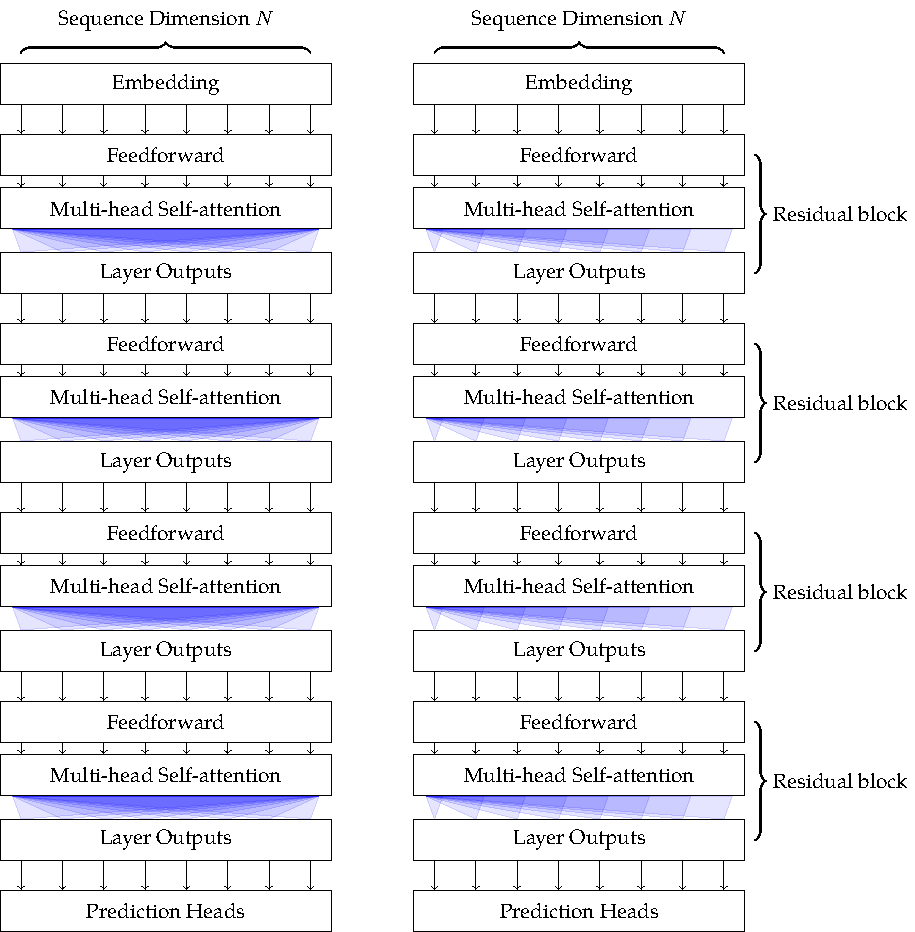
\includegraphics[width=1.2\linewidth]{figures/transformers.pdf}
    \caption[Transformer model]{Left: Encoder-only model. Right: Decoder-only model. Residual connections have been omitted for brevity.}
    \label{fig:transformers}
\end{figure}

\subsection{Encoder-decoder models}
\label[]{ss:encoder-decoder}

When the transformer was introduced in \cite{attention-is-all-you-need}, the first architecture proposed was an encoder-decoder architecture. This is a model which has both an encoder and a decoder. The encoder is used to encode a sequence of \textit{conditioning} or \textit{context} inputs, and the decoder is used to generate the output sequence. The encoder and decoder are connected by cross-attention layers (see \Cref{fig:cross-attn}), which allow the decoder to attend to the encoded context sequence.

Encoder-decoder models are more flexible than either previous class of model, because they allow predicting some outputs, or sequences of outputs, \textit{given} some inputs.

Examples of this are the original transformer architecture \cite{attention-is-all-you-need}, the BART \cite{bart} model, and more recently Google's Parti multi-modal text-to-image model \cite{parti}.

In \cite{attention-is-all-you-need}, they train an encoder-decoder architecture for text translation. Their architecture takes one sequence of text in language A as conditioning input, then auto-regressively samples a sequence of text in a second language B. The two languages can have very different word orderings or numbers of words to each other, and using the cross-attention operation to connect the two sequences introduces no bias towards aligned word orderings or even word counts.

\subsection{T5 models}

\begin{figure}
    \centering
    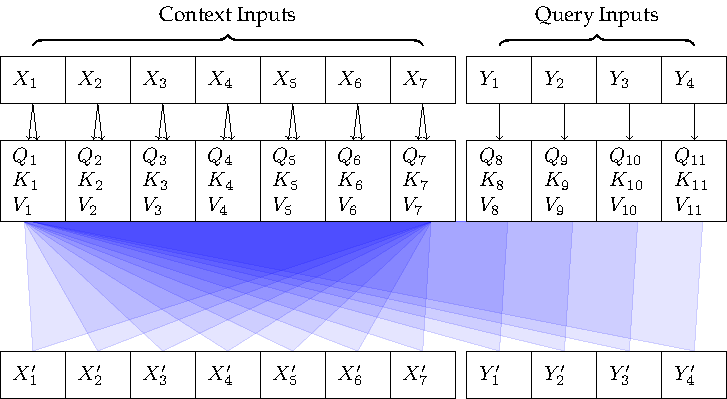
\includegraphics[]{figures/attn-5-unified.pdf}
    \captionsetup{parskip=7pt}
    \caption[Unified attention]{Unified self- and cross-attention, from \cite{unilm}.

    Bi- and uni-directional attention can be performed with the same attention layers with careful masking, allowing the same model to be trained on any mixture of pre-training tasks.

    The ``encoder'' outputs $X'$ are computed with full self-attention, and the ``decoder'' outputs $Y'$ are computed with full attention with respect to $X$ and causal attention with respect to $Y$.}
    \label{fig:unified-attn}
\end{figure}

The final commonly seen transformer architecture are T5 models \cite{t5}, which uses unified attention. As we saw before in \Cref{ss:unified}, we can use the same attention matrix for both the encoded sequence and the decoded sequence. However, as discussed, this is less computationally efficient than using cross attention. So, why would this be done?

The answer is that because a transformer shares weights across the sequence dimension, the resulting model will be capable of being used as either a bidirectional or unidirectional model, depending on the masking scheme used during inference. This is useful for \textit{transfer learning}, where we retrain (fine-tune) a model on a new, more specific task. Having a base model that has been trained with unified attention allows us to fine-tune the same model for both bidirectional and unidirectional tasks.

These models are known as T5 models: \textbf{T}ext-\textbf{T}o-\textbf{T}ext \textbf{T}ransfer \textbf{T}ransformers \cite{t5}. Training a large T5 model is very computationally expensive, but the resulting models are extremely useful for transfer learning. Currently, many state of the art results are being achieved by fine-tuning these models.

\section{Fast decoding}
\label{sec:fast-decoding}

\begin{figure}
    \centering
    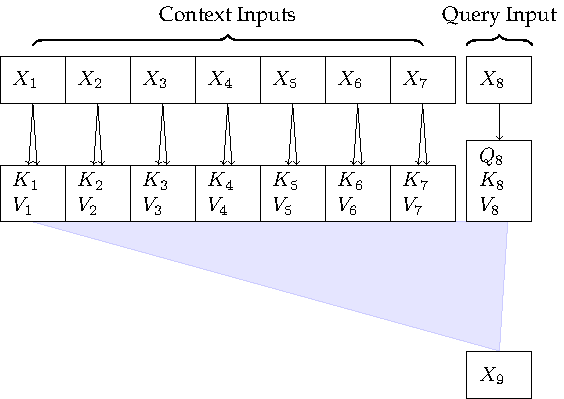
\includegraphics[]{figures/attn-4-partial.pdf}
    \caption[Partial self-attention]{Partial self-attention, as used during incremental autoregressive inference (in models with a decoder).}
    \label{fig:partial-self-attn}
\end{figure}

When training transformer models, an entire sequence of inputs is provided at once. However, at inference time not all the computations need to be performed to generate sequences. The computed key and value matrices can be reused for multiple predictions, and the attention matrices can be computed incrementally. When this is done attention operation looks as shown in \Cref{fig:partial-self-attn}.
